% Presentation for Inference-Time Guidance for Diffusion Policies
% Build with: make presentation (from project root)
% See paper/WORKFLOW.md for AI agent instructions

\documentclass[aspectratio=169]{beamer}
\usetheme{Madrid}
\usecolortheme{crane}

\usepackage{amsmath,amssymb,amsthm}
\usepackage{bm}
\usepackage{algorithm}
\usepackage{algorithmic}
\usepackage{tikz}
\usetikzlibrary{arrows,positioning,shapes,calc}
\usepackage{graphicx}
\usepackage{booktabs}
% \usepackage{animate}  % Requires complex dependencies, uncomment if needed
% \usepackage{multimedia}

% Path to figures
\graphicspath{{../figures/}}


% Custom colors
\definecolor{harvardcrimson}{RGB}{165,28,48}
\definecolor{softblue}{RGB}{65,105,225}
\definecolor{softgreen}{RGB}{34,139,34}
\definecolor{softorange}{RGB}{255,140,0}

\setbeamercolor{frametitle}{bg=harvardcrimson,fg=white}
\setbeamercolor{title}{bg=harvardcrimson,fg=white}
\setbeamercolor{structure}{fg=harvardcrimson}

\title{Compositional Model-Based Guidance\\for Diffusion Policies}
\subtitle{Inference-Time Planning in Online RL}
\author{Philip Nielsen}
\date{\today}
\institute{Harvard University}

\begin{document}

\maketitle

% =============================================================================
\section{Introduction}
% =============================================================================

\begin{frame}{Diffusion Policies for Reinforcement Learning}

\textbf{Diffusion policies} model action distributions as iterative denoising:
\[
a_T \sim \mathcal{N}(0, I) \;\to\; a_{T-1} \;\to\; \cdots \;\to\; a_0 \quad \text{(conditioned on state } s\text{)}
\]

\vspace{0.5em}
\textbf{Why diffusion for RL?}
\begin{itemize}
    \item Highly expressive: can model multimodal action distributions
    \item Stable training via simple denoising score matching
\end{itemize}

\vspace{0.5em}
\textbf{Challenge:} Standard diffusion training requires samples from the target distribution---but in online RL, we don't have samples from the \emph{optimal} policy.

\vspace{0.5em}
\textbf{Solution approaches:}
\begin{enumerate}
    \item \textbf{Training-time:} Reweight diffusion loss by Q-values (DPMD)
    \item \textbf{Inference-time:} Guide sampling toward high-value actions
\end{enumerate}

\end{frame}

% =============================================================================
\section{Guiding Diffusion Models}
% =============================================================================

\begin{frame}{Energy Guidance vs. Training-Free Guidance}

\textbf{Energy Guidance (General Case):}
Target a tilted distribution proportional to the base model times an energy term:
\[ \tilde{\pi}(a|s) \propto \pi_\theta(a|s) \cdot \exp(\lambda Q(s, a)) \]
\begin{itemize}
    \item Depends on an objective $Q$ trained on \emph{noisy} samples (actions).
    \item Allows for analytic expressions of the tilted distribution.
\end{itemize}

\vspace{0.5em}
\textbf{Training-Free Guidance (TFG):}
Relies on an objective $Q(s, a)$ trained only on \emph{clean} data.
\begin{itemize}
    \item $Q$ is a function of the \textbf{Tweedie estimate} of the clean action $\hat{a}_0(a_t)$.
    \item We take the gradient w.r.t. $a_t$ \textbf{through} this estimate:
    \[ \nabla_{a_t} Q(s, \hat{a}_0(a_t)) \]
\end{itemize}

\vspace{0.5em}
\textbf{The Trade-off:} With TFG, we lose the nice analytic exponential expression for the tilted distribution. Simple guidance no longer guarantees sampling from the optimal target.

\end{frame}

% =============================================================================
\begin{frame}{Recovering the Target Distribution with MCMC}

\textbf{Solution:} Define a sequence of \textbf{energy functions} at each noise level.

\vspace{0.5em}
The negative exponential of these energy functions is proportional to:
\begin{itemize}
    \item The \textbf{target distribution} at zero noise ($t=0$)
    \item The \textbf{standard normal} at full noise ($t=T$)
    \item A \textbf{smooth interpolation} between them at intermediate noise levels
\end{itemize}

\vspace{0.5em}
\textbf{Method (ULA/MALA):}
Apply MCMC methods at each noise level to match these intermediate distributions.

\vspace{0.5em}
$\implies$ If we match the distributions at each step, the sample distribution \textbf{smoothly converges} to the target distribution as the noise level approaches zero.

\end{frame}

% =============================================================================
\begin{frame}{MALA: Metropolis-Adjusted Langevin Algorithm}

\textbf{At each noise level $t$}, define energy:
\[
E_t(a_t) = E_{\text{model}}(a_t, s, t) - \lambda \cdot J(s, \hat{a}_0(a_t))
\]

\textbf{MALA update:}
\begin{enumerate}
    \item \textbf{Propose:} $a_t' = a_t - \eta \nabla_{a_t} E_t(a_t) + \sqrt{2\eta}\, z$, \quad $z \sim \mathcal{N}(0, I)$
    \item \textbf{Accept/Reject:} Metropolis-Hastings correction
    \[
    \text{Accept } a_t' \text{ w.p. } \min\left(1, \frac{q(a_t | a_t')}{q(a_t' | a_t)} e^{E_t(a_t) - E_t(a_t')}\right)
    \]
\end{enumerate}

\vspace{0.5em}
\textbf{Why MALA over plain Langevin (ULA)?}
\begin{itemize}
    \item MH correction removes discretization bias
    \item Guarantees convergence to correct distribution at each step
\end{itemize}

\end{frame}

% =============================================================================
\section{Compositional Q-Function}
% =============================================================================

\begin{frame}{Motivation for Replacing Q}

\textbf{Standard approach:} Use Q-function as the guidance objective
\[
J(s, a) = Q(s, a)
\]

\textbf{Issue:} Q-function depends on the current policy $\pi_\theta$:
\[
Q^\pi(s, a) = \mathbb{E}_\pi\left[\sum_{t=0}^\infty \gamma^t r_t \,\Big|\, s_0 = s, a_0 = a\right]
\]

\begin{itemize}
    \item As $\pi_\theta$ improves, $Q^\pi$ must be re-learned
    \item Q lags behind the policy $\Rightarrow$ stale guidance signal
    \item Q is learned via bootstrapping $\Rightarrow$ compounding errors
\end{itemize}

\vspace{0.5em}
\textbf{Question:} Can we build a guidance objective from components that are \emph{policy-independent} and learned via simple supervised learning?

\end{frame}

% =============================================================================
\begin{frame}{Compositional Objective: $r + \gamma V$}

\textbf{Key decomposition:}
\[
Q(s, a) = \mathbb{E}_{s' \sim p(\cdot|s,a)}\left[ r(s, a, s') + \gamma V(s') \right]
\]

\textbf{Learn each component separately:}

\begin{center}
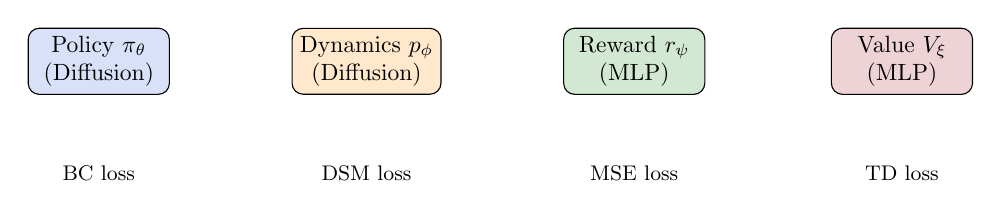
\begin{tikzpicture}[scale=0.85, every node/.style={scale=0.85},
    block/.style={rectangle, draw, rounded corners, minimum height=2.2em, minimum width=6em, text centered, align=center}]

\node[block, fill=softblue!20] (policy) at (0,0) {Policy $\pi_\theta$\\(Diffusion)};
\node[block, fill=softorange!20] (dynamics) at (4,0) {Dynamics $p_\phi$\\(Diffusion)};
\node[block, fill=softgreen!20] (reward) at (8,0) {Reward $r_\psi$\\(MLP)};
\node[block, fill=harvardcrimson!20] (value) at (12,0) {Value $V_\xi$\\(MLP)};

\node[below=0.8cm of policy] {\small BC loss};
\node[below=0.8cm of dynamics] {\small DSM loss};
\node[below=0.8cm of reward] {\small MSE loss};
\node[below=0.8cm of value] {\small TD loss};

\end{tikzpicture}
\end{center}

\vspace{0.5em}
\textbf{Advantages:}
\begin{itemize}
    \item \textbf{Dynamics \& Reward:} Pure supervised learning, no policy dependence
    \item \textbf{Value:} Still depends on $\pi$, but in multi-step planning, contribution decays as $\gamma^H$
    \item \textbf{Modularity:} Each component can be improved independently
\end{itemize}

\end{frame}

% =============================================================================
\begin{frame}{The Guidance Objective}

\textbf{At inference time}, compute:
\[
J(s, a) = \mathbb{E}_{s' \sim p_\phi(\cdot|s,a)}\left[ r_\psi(s, a, s') + \gamma V_\xi(s') \right]
\]

\textbf{Crucial:} The value function $V_\xi(s')$ is \textbf{required} to capture long-term returns; we have found it necessary for performance.

\vspace{0.5em}
\textbf{Monte Carlo estimation} with $N$ next-state particles:
\[
\hat{J}(s, a) = \frac{1}{N} \sum_{i=1}^{N} \left[ r_\psi(s, a, s'_i) + \gamma V_\xi(s'_i) \right], \quad s'_i \sim p_\phi(\cdot|s,a)
\]

\vspace{0.5em}
\textbf{For guidance}, we need:
\[
\nabla_{a_t} J(s, \hat{a}_0(a_t))
\]

This requires differentiating through:
\begin{enumerate}
    \item Dynamics model samples $s'_i$
    \item Reward and value networks
\end{enumerate}

\end{frame}

% =============================================================================
\section{The Algorithm}
% =============================================================================

\begin{frame}{Coupled Action-State Sampling}

\textbf{Challenge:} At each diffusion level $t$, we need fresh $s'$ samples given the current $\hat{a}_0$.

\vspace{0.5em}
\textbf{Solution:} Maintain a \textbf{population of $s'$ particles} that evolves alongside the action chain.

\vspace{0.8em}
% PLACEHOLDER FOR ANIMATION
\begin{center}
(animation)
\end{center}

\end{frame}

% =============================================================================
\begin{frame}{$s'$-Population Refresh (Recurrence)}

At each diffusion level $t$, given current clean estimate $\hat{a}_0$:

\vspace{0.5em}
\textbf{For} $\ell = 1, \ldots, L$ (refresh steps):
\begin{enumerate}
    \item Predict noise: $\hat{\epsilon} = \text{DynNet}_\phi(s, \hat{a}_0, s'_t, t)$
    \item Tweedie clean estimate: $\hat{s}'_0 = \frac{s'_t - \sqrt{1-\bar{\alpha}_t}\,\hat{\epsilon}}{\sqrt{\bar{\alpha}_t}}$
    \item Re-noise to level $t$: $s'_t \gets \sqrt{\bar{\alpha}_t}\,\hat{s}'_0 + \sqrt{1-\bar{\alpha}_t}\,\epsilon$, \quad $\epsilon \sim \mathcal{N}(0,I)$
\end{enumerate}

\vspace{0.5em}
\textbf{Effect:} Each recurrence step refines $s'$ particles while staying at noise level $t$.

\vspace{0.5em}
\textbf{Gradient flow:} For the last $B$ steps (``bprop refresh steps''), we allow gradients to flow through the recurrence---enabling the planner to ``steer'' the $s'$ population toward high-value regions.

\end{frame}

% =============================================================================
\begin{frame}{Full Inference Algorithm}

\begin{algorithmic}[1]
\small
\STATE \textbf{Input:} State $s$, models $(\pi_\theta, p_\phi, r_\psi, V_\xi)$, guidance strength $\lambda$
\STATE Initialize $a_T \sim \mathcal{N}(0, I)$, \; $\{s'_i\}_{i=1}^N \sim \mathcal{N}(0, I)$
\FOR{$t = T, T-1, \ldots, 1$}
    \STATE \textcolor{softblue}{\textbf{// Corrector: MALA refinement at noise level $t$}}
    \FOR{$k = 1, \ldots, K$}
        \STATE $\hat{a}_0 \gets \text{Tweedie}(a_t, \epsilon_\theta)$
        \STATE Refresh $\{s'_i\}$ via recurrence conditioned on $(s, \hat{a}_0)$
        \STATE $\hat{J} \gets \frac{1}{N}\sum_i [r_\psi(s, \hat{a}_0, s'_i) + \gamma V_\xi(s'_i)]$
        \STATE $E_t \gets E_{\text{model}}(a_t) - \lambda \cdot \hat{J}$
        \STATE $a_t \gets \text{MALA\_step}(a_t, \nabla_{a_t} E_t)$ \hfill \textit{// with $s'$ refresh in gradient}
    \ENDFOR
    \STATE \textcolor{softorange}{\textbf{// Predictor: Guided diffusion step}}
    \STATE $\nabla J \gets \nabla_{a_t} \hat{J}$ \hfill \textit{// reuse from last MALA step}
    \STATE $\epsilon_{\text{guided}} \gets \epsilon_\theta - \lambda \sigma_t \nabla J$
    \STATE $a_{t-1} \gets \text{DDPM\_step}(a_t, \epsilon_{\text{guided}})$
\ENDFOR
\STATE \textbf{Return:} $\text{clip}(a_0, -1, 1)$
\end{algorithmic}

\end{frame}

% =============================================================================
\begin{frame}{Training: Supervised Learning from Replay}

All components trained with simple losses on replay buffer $\mathcal{B}$:

\vspace{0.5em}
\textbf{Policy} (behavior cloning):
\[
\mathcal{L}_{\text{policy}} = \mathbb{E}_{(s,a) \sim \mathcal{B}, t, \epsilon}\left[ \| \epsilon_\theta(a_t, s, t) - \epsilon \|^2 \right]
\]

\textbf{Dynamics} (denoising score matching):
\[
\mathcal{L}_{\text{dyn}} = \mathbb{E}_{(s,a,s') \sim \mathcal{B}, t, \epsilon}\left[ \| \epsilon_\phi(s'_t, s, a, t) - \epsilon \|^2 \right]
\]

\textbf{Reward} (regression):
\[
\mathcal{L}_{\text{reward}} = \mathbb{E}_{(s,a,s',r) \sim \mathcal{B}}\left[ (r_\psi(s, a, s') - r)^2 \right]
\]

\textbf{Value} (TD learning):
\[
\mathcal{L}_{\text{value}} = \mathbb{E}_{(s,r,s') \sim \mathcal{B}}\left[ \left(V_\xi(s) - r - \gamma V_{\bar{\xi}}(s')\right)^2 \right]
\]

\end{frame}

% =============================================================================
\section{Results}
% =============================================================================

\begin{frame}{Toy Example: Exact Distribution Matching}

% PLACEHOLDER FOR PLOTS
\begin{center}
\includegraphics[width=.8\textheight]{action_match_pc_mala_fac_rr.png}\\[0.5em]
\end{center}

\vspace{0.5em}
\textbf{Key observation:} The MALA-corrected sampler with coupled $s'$-refresh correctly samples from the compositional objective.

\end{frame}

% =============================================================================
\begin{frame}{MuJoCo: HalfCheetah-v4}

% PLACEHOLDER FOR TRAINING CURVE
\begin{center}
\includegraphics[width=0.9\textwidth]{training_curve.png}\\[0.5em]
\end{center}

\begin{itemize}
    \item Diffusion policy with inference-time guidance
    \item Compositional model-based objective
    \item MALA correction with coupled state sampling
\end{itemize}
\ldots can learn \textbf{stably} in online RL setting.

\end{frame}

% =============================================================================
\begin{frame}{Scaling Dimensions for Future Work}

\textbf{Unlike vanilla Q-guided diffusion}, this approach opens multiple axes for scaling inference-time compute:

\vspace{0.5em}
\begin{itemize}
    \item \textbf{State population size} ($N$): More $s'$ particles $\to$ lower variance $\hat{J}$
    
    \item \textbf{MALA steps} ($K$): More correction steps $\to$ better convergence to tilted distribution
    
    \item \textbf{Refresh steps} ($L$): More recurrence $\to$ better $s'$ estimates
    
    \item \textbf{Planning horizon} ($H$): Multi-step rollouts $\to$ longer-horizon credit assignment
    \[
    J_H(s, a_0) = \mathbb{E}\left[\sum_{h=0}^{H-1} \gamma^h r_h + \gamma^H V(s_H)\right]
    \]
    
    \item \textbf{Action particles}: Sample multiple action chains, select best
\end{itemize}

\vspace{0.5em}
Each axis trades compute for potentially better action selection.

\end{frame}

% =============================================================================
\section{Summary}
% =============================================================================

\begin{frame}{Summary}

\textbf{Training-free guidance} enables tilting diffusion policies toward high-value actions using Tweedie estimates, but complicates exact sampling.

\vspace{0.5em}
\textbf{MCMC correction} (MALA) with a sequence of energy functions at each noise level recovers smooth convergence to the tilted distribution.

\vspace{0.5em}
\textbf{Compositional objective} $J = \mathbb{E}[r + \gamma V]$ replaces Q with:
\begin{itemize}
    \item Learned dynamics $p_\phi(s'|s,a)$
    \item Learned reward $r_\psi(s,a,s')$
    \item Learned value $V_\xi(s)$ (Crucial for performance)
\end{itemize}

\vspace{0.5em}
\textbf{Coupled sampling} of actions and next-states enables differentiable planning through the compositional objective.

\vspace{0.5em}
\textbf{Status:} Learns stably; multiple scaling axes for future improvement.

\end{frame}

% =============================================================================
% APPENDIX
% =============================================================================
\appendix

\begin{frame}{Appendix: Tweedie's Formula}

Given noisy observation $a_t = \sqrt{\bar{\alpha}_t}\, a_0 + \sqrt{1-\bar{\alpha}_t}\, \epsilon$:

\vspace{0.5em}
\textbf{Posterior mean} (Tweedie's formula):
\[
\mathbb{E}[a_0 | a_t] = \frac{a_t - \sqrt{1-\bar{\alpha}_t} \cdot \epsilon_\theta(a_t, t)}{\sqrt{\bar{\alpha}_t}}
\]

\vspace{0.5em}
This ``Tweedie estimate'' $\hat{a}_0$ lets us:
\begin{itemize}
    \item Query clean-data objectives: $r(s, \hat{a}_0, s')$, $V(s')$
    \item Condition the dynamics model: $p_\phi(s' | s, \hat{a}_0)$
    \item Compute guidance gradients: $\nabla_{a_t} J(s, \hat{a}_0(a_t))$
\end{itemize}

\vspace{0.5em}
The gradient flows through $\hat{a}_0$ because:
\[
\frac{\partial \hat{a}_0}{\partial a_t} = \frac{1}{\sqrt{\bar{\alpha}_t}}\left(I - \sqrt{1-\bar{\alpha}_t} \cdot \frac{\partial \epsilon_\theta}{\partial a_t}\right)
\]

\end{frame}

% =============================================================================
\begin{frame}{Appendix: Energy Parameterization}

\textbf{Standard diffusion:} Network predicts noise $\epsilon_\theta(a_t, s, t)$

\textbf{Energy parameterization:} Network predicts scalar energy $E_\theta(a_t, s, t)$
\[
\epsilon_\theta(a_t, s, t) = \nabla_{a_t} E_\theta(a_t, s, t)
\]

\vspace{0.5em}
\textbf{Advantage:} Explicit energy enables:
\begin{itemize}
    \item Metropolis-Hastings acceptance ratios (need $e^{-E}$ not just $\nabla E$)
    \item Principled composition of energies
    \item Exact sampling via MCMC
\end{itemize}

\vspace{0.5em}
\textbf{Combined energy for MALA:}
\[
E_{\text{total}}(a_t) = E_\theta(a_t, s, t) - \lambda \cdot \mathbb{E}_{s'}\left[r(s, \hat{a}_0, s') + \gamma V(s')\right]
\]

This ensures MALA and diffusion guidance target the same tilted distribution.

\end{frame}

% =============================================================================
\begin{frame}{Appendix: Why Recurrence for $s'$ Refresh?}

\textbf{Problem:} At diffusion level $t$, we need $s' \sim p(s'|s, \hat{a}_0)$, but $\hat{a}_0$ changes as $a_t$ is refined.

\vspace{0.5em}
\textbf{Naive approach:} Sample fresh $s'$ particles from scratch at each step.
\begin{itemize}
    \item Expensive: full $T$-step diffusion rollout
    \item Discontinuous: $s'$ population ``jumps'' between steps
\end{itemize}

\vspace{0.5em}
\textbf{Recurrence approach:} Stay at noise level $t$ and iteratively refine:
\[
s'_t \;\xrightarrow{\text{Tweedie}}\; \hat{s}'_0 \;\xrightarrow{\text{re-noise}}\; s'_t
\]

\begin{itemize}
    \item Cheap: just a few network evaluations per refresh
    \item Smooth: $s'$ population evolves continuously with $a_t$
    \item Differentiable: gradients flow through the recurrence
\end{itemize}

\end{frame}

\end{document}
